\chapter{Experiment Results} \label{secEXP}
\section{Datasets and Implementation}

\textbf{Pascal Visual Object Classes Challenge 2012 (VOC2012) \cite{pascal-voc-2012}.} This famous object detection benchmark consists of 20 classes. We use this dataset to show our work's capability in reducing computing time. Training set and validation set are used to train models while the test set is used to evaluate performance. Notice that this dataset only has a relative small number of classes but the experiment result proves that we can perform well on it. In Figure. \ref{figFeatureUsage}...

\begin{figure}
\centering
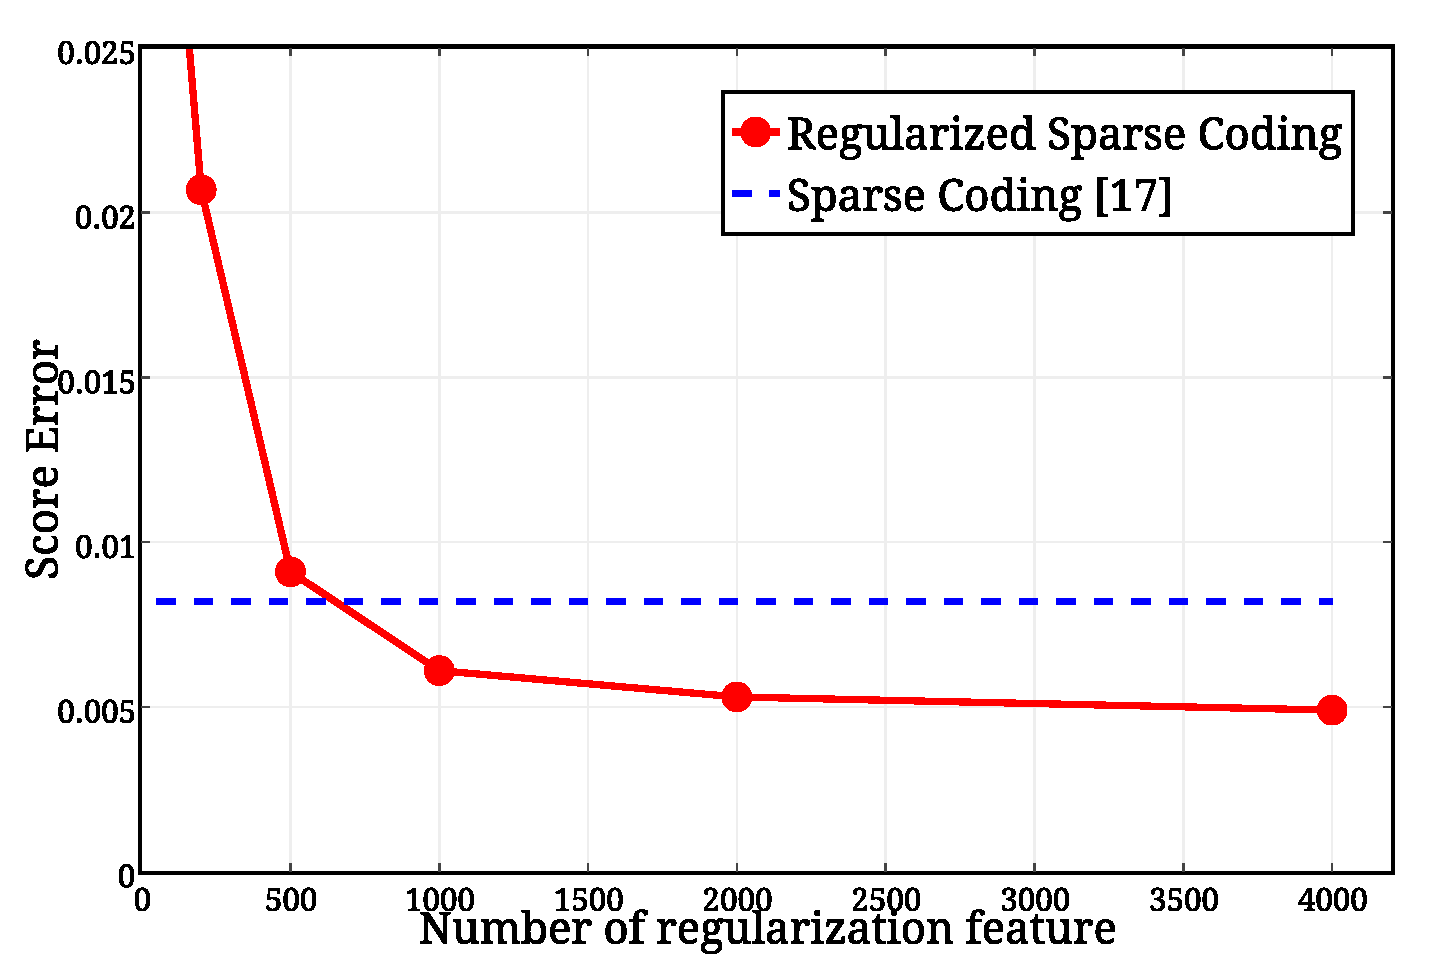
\includegraphics[width=0.48\textwidth]{featureUsage}
\caption{Effect of the number of regularization features used in Regularized Sparse Coding\protect\footnotemark[3]. As the solid line illustrates, the score error drops with more features involved. The dotted line is the original sparse coding method. Although sparse coding also has low score error, small difference of score error between the two method will result in a huge performance difference (mAP) in later experiments.}
\label{figFeatureUsage}
\end{figure}

\section{Performance Analysis}

\section{Scalability}

To compare sparse coding with our method, we conduct experiments on ILSVRC2013 ...

